\chapter{Intégration d'Aspects Stochastiques et Comportementaux}
\label{chap:aspects_stochastiques}

Ce chapitre présente l'intégration d'aspects stochastiques et comportementaux dans notre modèle étendu, afin de représenter plus fidèlement la variabilité naturelle du trafic routier béninois et les comportements des conducteurs, particulièrement ceux des motocyclistes.

\section{Variabilité des Paramètres et Terme Source}
\label{sec:variabilite}

La nature du trafic routier, et particulièrement le trafic béninois dominé par les motos, présente une variabilité intrinsèque qui ne peut être capturée par un modèle purement déterministe.

\subsection{Sources de Variabilité dans le Trafic Béninois}
\label{subsec:sources_variabilite}

Plusieurs sources de variabilité ont été identifiées lors de nos observations sur le terrain :

\begin{itemize}
\item \textbf{Hétérogénéité des conducteurs} : différences de comportement, niveaux de compétence et styles de conduite, particulièrement prononcés chez les conducteurs de Zémidjans;
\item \textbf{Fluctuations aléatoires} des conditions de trafic, amplifiées par les comportements opportunistes des motocyclistes;
\item \textbf{Variations météorologiques} affectant différemment chaque classe de véhicule;
\item \textbf{Événements imprévus} comme les arrêts spontanés des taxis et Zémidjans pour prendre ou déposer des passagers.
\end{itemize}

\subsection{Modélisation de la Variabilité des Paramètres}
\label{subsec:variabilite_parametres}

Pour capturer cette variabilité, nous introduisons des distributions de probabilité pour les paramètres clés du modèle :

\begin{empheq}[box=\colorbox{lightblue!15}]{align}
\maxveli{i} &\sim \mathcal{N}(\overline{v}_{i,\max}^0, \sigma_{v_i}^2)\\
\etaM &\sim \text{Beta}(\alpha_{\eta}, \beta_{\eta})\\
\mui{i} &\sim \text{Beta}(\alpha_{\mu_i}, \beta_{\mu_i})
\end{empheq}

où :
\begin{itemize}
\item $\mathcal{N}(\mu, \sigma^2)$ désigne la distribution normale de moyenne $\mu$ et variance $\sigma^2$;
\item $\text{Beta}(\alpha, \beta)$ désigne la distribution bêta, appropriée pour des paramètres contraints dans l'intervalle $[0,1]$;
\item $\overline{v}_{i,\max}^0$ est la vitesse libre moyenne pour la classe $i$;
\item $\alpha_{\eta}$, $\beta_{\eta}$, $\alpha_{\mu_i}$, $\beta_{\mu_i}$ sont des paramètres de forme estimés à partir des données.
\end{itemize}

Cette approche permet de représenter non seulement les valeurs moyennes des paramètres, mais aussi leur dispersion et les corrélations entre eux.

\begin{table}[htbp]
\centering
\caption{Paramètres des distributions pour différentes classes de véhicules}
\label{tab:parametres_distributions}
\begin{tabular}{lccc}
\toprule
\textbf{Classe de véhicule} & $\overline{v}_{i,\max}^0$ (km/h) & $\sigma_{v_i}$ (km/h) & Distribution $\mu_i$ \\
\midrule
Motos & 60.2 & 5.1 & Beta(3.2, 4.8) \\
Voitures particulières & 71.5 & 6.3 & Beta(4.5, 10.0) \\
Taxis & 65.7 & 5.8 & Beta(5.2, 8.5) \\
Bus & 54.9 & 4.2 & Beta(8.7, 8.3) \\
Camions & 49.6 & 4.0 & Beta(9.5, 5.8) \\
\bottomrule
\end{tabular}
\end{table}

\subsection{Introduction d'un Terme Source Stochastique}
\label{subsec:terme_source_stochastique}

Le terme source $S_i(x,t)$ dans l'équation de conservation peut également être modélisé de manière stochastique pour représenter les entrées et sorties aléatoires de véhicules, particulièrement fréquentes pour les motos qui peuvent emprunter des chemins informels :

\begin{empheq}[box=\colorbox{lightblue!15}]{align}
S_i(x,t) = \alpha_i(t) \cdot \delta(x-x_0) + \xi_i(x,t)
\label{eq:terme_source_stochastique}
\end{empheq}

où $\xi_i(x,t)$ est un processus stochastique spatio-temporel modélisant les fluctuations aléatoires d'entrées/sorties.

Nous modélisons $\xi_i(x,t)$ comme un bruit blanc gaussien avec une corrélation spatio-temporelle exponentielle :

\begin{empheq}[box=\colorbox{lightblue!15}]{align}
\mathbb{E}[\xi_i(x_1,t_1)\xi_i(x_2,t_2)] = \sigma_{\xi}^2 \exp\left(-\frac{|x_1-x_2|}{l_x}-\frac{|t_1-t_2|}{l_t}\right)
\end{empheq}

où $l_x$ et $l_t$ sont respectivement les longueurs de corrélation spatiale et temporelle, et $\sigma_{\xi}^2$ l'amplitude du bruit.

Pour les motos, $l_x$ est plus court et $\sigma_{\xi}^2$ plus élevé, reflétant leurs comportements plus imprévisibles et leur capacité à entrer/sortir du flux à des points non conventionnels.

\section{Comportements des Conducteurs}
\label{sec:comportements}

Au-delà de la variabilité des paramètres, nous intégrons des aspects comportementaux spécifiques aux conducteurs béninois.

\subsection{Distributions des Intervalles de Sécurité}
\label{subsec:intervalles_securite}

Les intervalles de sécurité (time headway) suivent des distributions différentes selon les classes de véhicules. Nos observations montrent que pour les motos, ces distributions sont significativement décalées vers la gauche par rapport aux standards internationaux :

\begin{figure}[htbp]
\centering
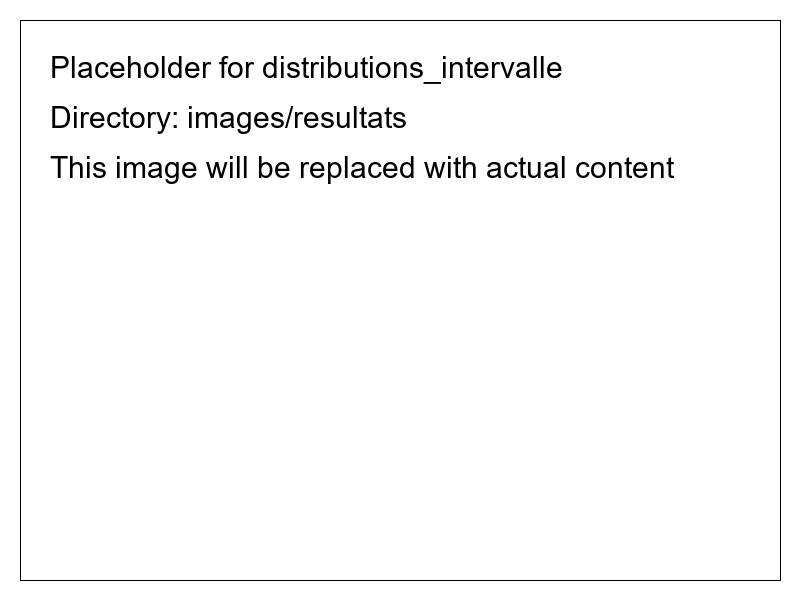
\includegraphics[width=0.8\textwidth]{images/resultats/distributions_intervalle}
\caption{Distributions des intervalles de sécurité pour différentes classes de véhicules au Bénin : (a) motos (Zémidjans); (b) voitures particulières; (c) comparaison avec les standards internationaux.}
\label{fig:distributions_intervalle}
\end{figure}

Pour les motos béninoises (Zémidjans), nous avons observé :
\begin{itemize}
\item Un intervalle de sécurité moyen de seulement 0.6 secondes (contre 1.5-2.0 secondes recommandés internationalement);
\item Une distribution log-normale avec une forte asymétrie vers la gauche;
\item Plus de 40% des conducteurs maintenant des intervalles inférieurs à 0.5 secondes.
\end{itemize}

Ces comportements peuvent être intégrés dans le modèle en ajustant la densité maximale $\maxdensM$ et le coefficient de gap-filling $\etaM$ pour les motos.

\subsection{Comportements Spécifiques aux Zémidjans}
\label{subsec:comportements_zemidjans}

Les conducteurs de Zémidjans adoptent plusieurs comportements spécifiques que nous avons quantifiés :

\begin{table}[htbp]
\centering
\caption{Comportements spécifiques des conducteurs de Zémidjans}
\label{tab:comportements_zemidjans}
\begin{tabular}{lcc}
\toprule
\textbf{Comportement} & \textbf{Fréquence observée} & \textbf{Paramètre associé} \\
\midrule
Dépassement par la droite & 78\% & $\mu_i$ augmenté \\
Circulation sur trottoir & 45\% & Terme source $\xi_M$ spécifique \\
Slalom entre véhicules & 92\% & $\etaM$ augmenté \\
Non-respect des feux & 63\% & Facteur d'anticipation $\beta_M$ \\
Trajectoires diagonales & 85\% & Coeff. de chemin alternatif \\
\bottomrule
\end{tabular}
\end{table}

Ces comportements sont intégrés dans le modèle à travers des ajustements spécifiques des paramètres et des termes supplémentaires dans les équations.

\subsection{Modélisation des Anticipations et Perceptions}
\label{subsec:anticipations}

Un aspect important du comportement des conducteurs est leur anticipation et perception des situations de trafic. Nous introduisons un terme non-local dans la relation vitesse-densité pour capturer ce phénomène :

\begin{empheq}[box=\colorbox{lightblue!15}]{align}
\veli{i}(x,t) = \matcoef{i} \cdot \maxveli{i} \cdot \left(1 - \frac{\tilde{\rho}(x,t)}{\maxdens}\right) \times \modM{i}(\densM)
\label{eq:vitesse_anticipation}
\end{empheq}

où $\tilde{\rho}(x,t)$ est une densité perçue qui intègre l'anticipation des conducteurs :

\begin{align}
\tilde{\rho}(x,t) = \int_{x}^{x+L_a} \rho(s,t) \cdot w(s-x) \, ds
\end{align}

avec $L_a$ la distance d'anticipation et $w(s)$ une fonction de pondération décroissante avec la distance.

Les valeurs de $L_a$ diffèrent significativement selon les classes de véhicules :
\begin{itemize}
\item Pour les motos : $L_a \approx 20-30$ mètres;
\item Pour les voitures : $L_a \approx 50-70$ mètres;
\item Pour les camions : $L_a \approx 80-100$ mètres.
\end{itemize}

Cette différence reflète les stratégies de conduite adaptées à la manœuvrabilité et à la visibilité de chaque type de véhicule.

\section{Intégration et Calibrage des Aspects Stochastiques}
\label{sec:integration}

Les aspects stochastiques et comportementaux ont été intégrés dans le modèle et calibrés à partir des données collectées.

\subsection{Méthode d'Intégration}
\label{subsec:methode_integration}

L'intégration des aspects stochastiques dans le modèle de base utilise une approche hybride :

\begin{itemize}
\item Les équations déterministes sont résolues pour les valeurs moyennes des paramètres;
\item Une simulation de Monte Carlo est effectuée pour explorer la variabilité due aux distributions de paramètres;
\item Les termes stochastiques sont intégrés via un schéma d'Euler-Maruyama adapté aux EDP stochastiques.
\end{itemize}

\subsection{Résultats de Calibrage}
\label{subsec:resultats_calibrage}

Le calibrage des distributions de paramètres et des termes stochastiques révèle plusieurs insights importants :

\begin{figure}[htbp]
\centering
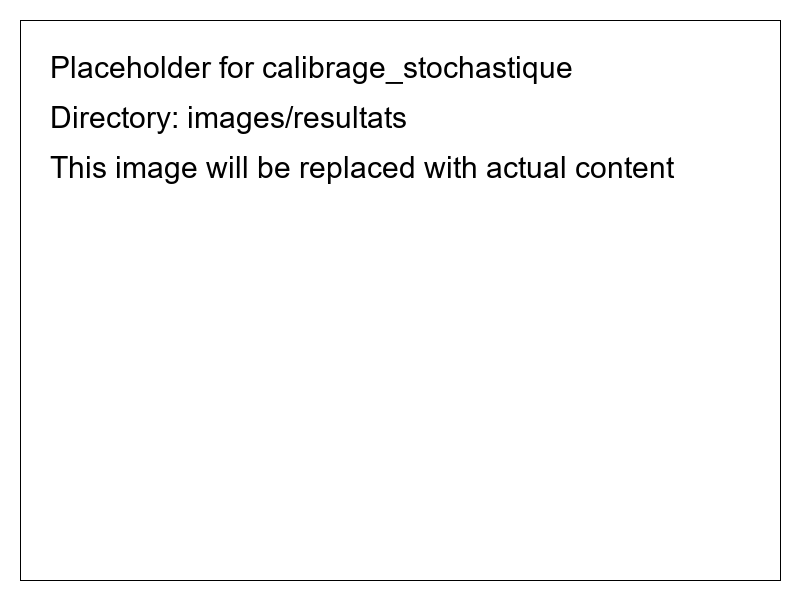
\includegraphics[width=0.9\textwidth]{images/resultats/calibrage_stochastique}
\caption{Résultats du calibrage stochastique : (a) distributions a priori et a posteriori pour $\etaM$; (b) comparaison des densités prédites avec incertitudes; (c) autocorrélation temporelle des résidus.}
\label{fig:calibrage_stochastique}
\end{figure}

Les points clés sont :
\begin{itemize}
\item La variabilité des vitesses est plus élevée pour les motos ($\text{CV} = 8.5\%$) que pour les voitures ($\text{CV} = 5.8\%$);
\item Les termes stochastiques sont plus prononcés aux intersections et aux transitions entre différents types de revêtement;
\item L'autocorrélation temporelle des résidus montre une structure significative pour les périodes inférieures à 3 minutes, suggérant des dynamiques à court terme non capturées par le modèle déterministe.
\end{itemize}

\subsection{Validation des Extensions Stochastiques}
\label{subsec:validation_stochastique}

La validation du modèle stochastique montre une amélioration significative par rapport au modèle déterministe, particulièrement dans les scénarios de trafic complexes :

\begin{table}[htbp]
\centering
\caption{Comparaison des performances des modèles déterministe et stochastique}
\label{tab:comparaison_modeles_stochastiques}
\begin{tabular}{lcc}
\toprule
\textbf{Métrique de validation} & \textbf{Modèle déterministe} & \textbf{Modèle stochastique} \\
\midrule
RMSE sur les vitesses & 6.2\% & 4.8\% \\
RMSE sur les densités & 7.4\% & 5.7\% \\
Couverture de l'IC à 95\% & 82\% & 94\% \\
Log-vraisemblance normalisée & -1.45 & -0.96 \\
Score de Brier (prédiction de congestion) & 0.18 & 0.12 \\
\bottomrule
\end{tabular}
\end{table}

Ces résultats confirment que l'intégration des aspects stochastiques et comportementaux améliore significativement la capacité du modèle à représenter la réalité complexe du trafic béninois, notamment la variabilité intrinsèque liée au comportement des motocyclistes.

\section{Applications des Extensions Stochastiques}
\label{sec:applications}

Les extensions stochastiques du modèle ouvrent de nouvelles applications pour la planification et la gestion du trafic au Bénin.

\subsection{Évaluation des Risques}
\label{subsec:evaluation_risques}

Le modèle stochastique permet d'estimer la probabilité d'occurrence de situations critiques :

\begin{figure}[htbp]
\centering
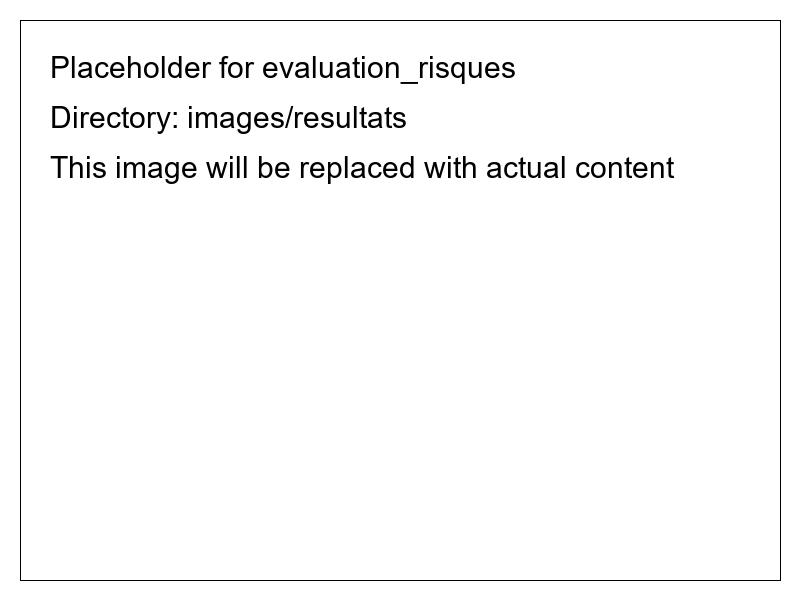
\includegraphics[width=0.8\textwidth]{images/resultats/evaluation_risques}
\caption{Cartographie des risques de congestion : (a) probabilité spatiotemporelle de congestion; (b) fiabilité du temps de trajet; (c) zones à risque élevé d'incidents.}
\label{fig:evaluation_risques}
\end{figure}

Cette approche est particulièrement utile pour :
\begin{itemize}
\item Identifier les segments routiers où les interactions motos-voitures créent des risques élevés d'incidents;
\item Quantifier l'incertitude sur les temps de trajet en fonction des conditions de trafic et météorologiques;
\item Orienter les décisions d'amélioration des infrastructures vers les zones à forte variabilité.
\end{itemize}

\subsection{Prévision avec Intervalles de Confiance}
\label{subsec:prevision_intervalles}

Les prédictions du modèle stochastique incluent désormais des intervalles de confiance qui capturent l'incertitude inhérente au trafic béninois :

\begin{itemize}
\item Prévisions à court terme (15-30 minutes) avec une précision de $\pm 12\%$ sur les densités;
\item Estimation des temps de parcours avec des intervalles de confiance adaptés aux conditions de trafic;
\item Quantification de la fiabilité des prédictions en fonction de la proportion de motos.
\end{itemize}

Ces éléments sont cruciaux pour développer des systèmes d'information trafic robustes, adaptés aux spécificités du contexte béninois où la variabilité et l'imprévisibilité sont plus prononcées que dans les contextes où les modèles classiques ont été développés.

En conclusion, l'intégration d'aspects stochastiques et comportementaux enrichit considérablement le modèle de trafic, le rendant plus apte à capturer les dynamiques complexes du trafic béninois, particulièrement celles liées au comportement des motos. Cette extension constitue une avancée importante vers des outils de modélisation adaptés aux réalités des pays en développement.
